\tikzset{
	A/.pic={
        code={
\draw[black](0,0)node[rotate=00]{\tiny \texttt{A}};
\draw[black,thick](-0.5,-0.15)rectangle(0.5,0.15);   
							}
	}
}

\tikzset{
	B/.pic={
        code={
\draw[black](0,0)node[rotate=00]{\tiny \texttt{B}};
\draw[black,thick](-0.5,-0.15)rectangle(0.5,0.15);   
							}
	}
}

\tikzset{
	C/.pic={
        code={
\draw[black](0,0)node[rotate=00]{\tiny \texttt{C}};
\draw[black,thick](-0.5,-0.15)rectangle(0.5,0.15);   
							}
	}
}

\tikzset{
	D/.pic={
        code={
\draw[black](0,0)node[rotate=00]{\tiny \texttt{D}};
\draw[black,thick](-0.5,-0.15)rectangle(0.5,0.15);   
							}
	}
}

\tikzset{
	main/.pic={
        code={
\draw[black](0,0)node[rotate=00]{\tiny \texttt{main}};
\draw[black,thick](-0.5,-0.15)rectangle(0.5,0.15);   
							}
	}
}

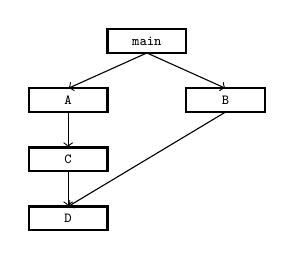
\begin{tikzpicture}
%Gitter
%\draw[step=0.5cm,very thin,black!20] (-6,-6) grid(6,6);
%\draw(-6,0)--(6,0);
%\draw(0,6)--(0,-6);
\path (0,2.75) pic {main};
\path (-1,2) pic {A};
\path (1,2) pic {B};
\path (-1,1.25) pic {C};
\path (-1,0.5) pic {D};
\draw [black,->] (0,2.6)--(-1,2.15);
\draw [black,->] (0,2.6)--(1,2.15);
\draw [black,->] (-1,1.85)--(-1,1.4);
\draw [black,->] (-1,1.1)--(-1,0.65);
\draw [black,->] (1,1.85)--(-1,0.65);
\end{tikzpicture}
